\documentclass[paper=letter,11pt]{scrartcl}

\KOMAoptions{headinclude=true, footinclude=false}
\KOMAoptions{DIV=14, BCOR=5mm}
\KOMAoptions{numbers=noendperiod}
\KOMAoptions{parskip=half}
\addtokomafont{disposition}{\rmfamily}
\addtokomafont{part}{\LARGE}
\addtokomafont{descriptionlabel}{\rmfamily}
%\setkomafont{pageheadfoot}{\normalsize\sffamily}
\setkomafont{pagehead}{\normalsize\rmfamily}
%\setkomafont{publishers}{\normalsize\rmfamily}
\setkomafont{caption}{\normalfont\small}
\setcapindent{0pt}
\deffootnote[1em]{1em}{1em}{\textsuperscript{\thefootnotemark}\ }


\usepackage{amsmath}
\usepackage[varg]{txfonts}
\usepackage[T1]{fontenc}
\usepackage{graphicx}
\usepackage{xcolor}
\usepackage[american]{babel}
% hyperref is needed in many places, so include it here
\usepackage{hyperref}

\usepackage{xspace}
\usepackage{multirow}
\usepackage{float}


\usepackage{braket}
\usepackage{bbm}
\usepackage{relsize}
\usepackage{tcolorbox}

\def\ketY{\ensuremath{\ket {\Psi}}}
\def\iGeV{\ensuremath{\textrm{GeV}^{-1}}}
%\def\mp{\ensuremath{m_{\textrm{proton}}}}
\def\rp{\ensuremath{r_{\textrm{proton}}}}
\def\me{\ensuremath{m_{\textrm{electron}}}}
\def\aG{\ensuremath{\alpha_G}}
\def\rAtom{\ensuremath{r_{\textrm{atom}}}}
\def\rNucl{\ensuremath{r_{\textrm{nucleus}}}}
\def\GN{\ensuremath{\textrm{G}_\textrm{N}}}
\def\ketX{\ensuremath{\ket{\vec{x}}}}
\def\ve{\ensuremath{\vec{\epsilon}}}


\def\ABCDMatrix{\ensuremath{\begin{pmatrix} A &  B  \\ C  & D \end{pmatrix}}}
\def\xyprime{\ensuremath{\begin{pmatrix} x' \\ y' \end{pmatrix}}}
\def\xyprimeT{\ensuremath{\begin{pmatrix} x' &  y' \end{pmatrix}}}
\def\xy{\ensuremath{\begin{pmatrix} x \\ y \end{pmatrix}}}
\def\xyT{\ensuremath{\begin{pmatrix} x & y \end{pmatrix}}}

\def\IMatrix{\ensuremath{\begin{pmatrix} 0 &  1  \\ -1  & 0 \end{pmatrix}}}
\def\IBoostMatrix{\ensuremath{\begin{pmatrix} 0 &  1  \\ 1  & 0 \end{pmatrix}}}
\def\JThree{\ensuremath{\begin{pmatrix}    0 & -i & 0  \\ i & 0  & 0 \\ 0 & 0 & 0 \end{pmatrix}}} 
\def\JTwo{\ensuremath{\begin{bmatrix}    0 & 0 & -i  \\ 0 & 0  & 0 \\ i & 0 & 0 \end{bmatrix}}}
\def\JOne{\ensuremath{\begin{bmatrix}    0 & 0 & 0  \\ 0 & 0  & -i \\ 0 & i & 0 \end{bmatrix}}}
\def\etamn{\ensuremath{\eta_{\mu\nu}}}
\def\Lmn{\ensuremath{\Lambda^\mu_\nu}}
\def\dmn{\ensuremath{\delta^\mu_\nu}}
\def\wmn{\ensuremath{\omega^\mu_\nu}}
\def\be{\begin{equation*}}
\def\ee{\end{equation*}}
\def\bea{\begin{eqnarray*}}
\def\eea{\end{eqnarray*}}
\def\bi{\begin{itemize}}
\def\ei{\end{itemize}}
\def\fmn{\ensuremath{F_{\mu\nu}}}
\def\fMN{\ensuremath{F^{\mu\nu}}}
\def\bc{\begin{center}}
\def\ec{\end{center}}
\def\nus{$\nu$s}

\def\adagger{\ensuremath{a_{p\sigma}^\dagger}}
\def\lineacross{\noindent\rule{\textwidth}{1pt}}

\newcommand{\multiline}[1] {
\begin{tabular} {|l}
#1
\end{tabular}
}

\newcommand{\multilineNoLine}[1] {
\begin{tabular} {l}
#1
\end{tabular}
}



\newcommand{\lineTwo}[2] {
\begin{tabular} {|l}
#1 \\
#2
\end{tabular}
}

\newcommand{\rmt}[1] {
\textrm{#1}
}


%
% Units
%
\def\m{\ensuremath{\rmt{m}}}
\def\GeV{\ensuremath{\rmt{GeV}}}
\def\pt{\ensuremath{p_\rmt{T}}}


\def\parity{\ensuremath{\mathcal{P}}}

\usepackage{cancel}
\usepackage{ mathrsfs }
\def\bigL{\ensuremath{\mathscr{L}}}

\usepackage{ dsfont }



\usepackage{fancyhdr}
\fancyhf{}

%\documentclass[margin,line]{res}
\usepackage{braket}
\usepackage{bbm}
\usepackage{relsize}

\def\ketY{\ensuremath{\ket {\Psi}}}
\def\iGeV{\ensuremath{\textrm{GeV}^{-1}}}


\def\ABCDMatrix{\ensuremath{\begin{pmatrix} A &  B  \\ C  & D \end{pmatrix}}}
\def\xyprime{\ensuremath{\begin{pmatrix} x' \\ y' \end{pmatrix}}}
\def\xyprimeT{\ensuremath{\begin{pmatrix} x' &  y' \end{pmatrix}}}
\def\xy{\ensuremath{\begin{pmatrix} x \\ y \end{pmatrix}}}
\def\xyT{\ensuremath{\begin{pmatrix} x & y \end{pmatrix}}}

\def\IMatrix{\ensuremath{\begin{pmatrix} 0 &  1  \\ -1  & 0 \end{pmatrix}}}
\def\IBoostMatrix{\ensuremath{\begin{pmatrix} 0 &  1  \\ 1  & 0 \end{pmatrix}}}
\def\JThree{\ensuremath{\begin{pmatrix}    0 & -i & 0  \\ i & 0  & 0 \\ 0 & 0 & 0 \end{pmatrix}}} 
\def\JTwo{\ensuremath{\begin{bmatrix}    0 & 0 & -i  \\ 0 & 0  & 0 \\ i & 0 & 0 \end{bmatrix}}}
\def\JOne{\ensuremath{\begin{bmatrix}    0 & 0 & 0  \\ 0 & 0  & -i \\ 0 & i & 0 \end{bmatrix}}}
\def\etamn{\ensuremath{\eta_{\mu\nu}}}
\def\Lmn{\ensuremath{\Lambda^\mu_\nu}}
\def\dmn{\ensuremath{\delta^\mu_\nu}}
\def\wmn{\ensuremath{\omega^\mu_\nu}}
\def\be{\begin{equation*}}
\def\ee{\end{equation*}}
\def\nus{$\nu$s}
%\def\xMu{\ensuremath{x^\mu}

\usepackage{fancyhdr}

\fancyhf{}
\lhead{\Large 33-444} % \hfill Introduction to Particle Physics \hfill Spring 2019}
\chead{\Large Introduction to Particle Physics} % \hfill Spring 2019}
\rhead{\Large Spring 2019} % \hfill Introduction to Particle Physics \hfill Spring 2019}

\begin{document}
\thispagestyle{fancy}

\begin{center}
{\huge \textbf{Lecture 31}}
\end{center}

{\fontsize{14}{16}\selectfont

\textbf{\underline{Neutrino Physics}} 

Will now switch gears and spend a few lectures focused on neutrino physics. 

Here is the Big picture for the next week or so...

\begin{itemize}
\item[-] Start with background of the physics of $\nu$s
\item[-] History of how we got to today (Brief.)
\item[-] Talk about what used to be called the ``Neutrino Puzzles''\\
          (This is ultimately the reason \nus\ are more interesting that we once thought. Major outcome will be that Neutrinos have mass)
\item[-] Neutrino Oscillations (Physics associated to $\nu$ mass)
\item[-] Where we are now and where we want to go.
\item[-] Neutrino masses as physics beyond the Standard Model\\
\end{itemize}

There is lots that we wont be covering (eg: \nus\ in astrophysics and cosmology ect. )

\vspace*{0.4in}

That is the plan... Questions ?

\vspace*{0.2in}

\noindent\rule{\textwidth}{1pt}

\textbf{\underline{Teasers}} (Neutrinos play an important role in the Universe)

\begin{itemize}
\item[-] $10^9:1$ Ratio of \nus\ to the other known particles (e,p,n)
\item[-] $\sim400/cm^3$ density of relic \nus\ from the Big Bang.
\item[-] $99\%$ fraction of E carried away by \nus\ in a Supernova
\item[-] $10^{38}$ \nus/s produced by the sun $\Rightarrow$ $10^{11}$ \nus/($cm^2s$)
\item[-] $10^6$ \nus/day produced by a banana from radioactive Potassium
\end{itemize}

\clearpage

Start by talking a little bit about how we got here.

\textbf{\underline{Brief History} } 

(Will actually start with the Pre-History. Note: not comprehensive, cherry-picked history for our discussion) 

\textbf{Story starts in 1896 w/Henri Becquerel}
Studying phosphorescence in Uranium salts. Expose sample and see how it behaves afterwards.  
In Paris (probably) they had a long spell of bad weather and saw that the salts activated photographic plates even when not exposed to light

Very surprising. There are some materials that emit stuff when just sitting there.

Opened a huge industry of studying radioactivity.

Found three types of radiation which they could then classify in terms of various properties. 

(Remember all this is happening before QM) 

Could ask what the radiation does in a magnetic field, what happens when you try to shield it ... that's basically it.

\begin{tabular}{l}
$\alpha$ radiation $\Rightarrow$ +  / Easy to stop\\
$\beta$ radiation $\Rightarrow$ -  / Harder to stop \\
$\gamma$ radiation $\Rightarrow$ 0 / Very hard to stop \\
\end{tabular}

\textbf{Once you get good at experiments you can ask what is the energy of the radiation that comes out.}

Remember this is all very \underline{weird} stuff: Material that just spits out energy w/out being excited.

Turns out, if you look at $\alpha$ or $\gamma$ radiation, there is a well-defined energy that comes out. 

We will be mainly concerned with $\beta$ radiation, which has a long and very interesting history. (which we wont go into) 

Real challenge was with the spectrum of $\beta$-radiation. 
Was it Continuous or Discrete ?
Naive expectation is that you would get a bunch of discrete lines.  

\textit{Why ?}  ``This is what spectra look like'' / ``This is what they do''

Experimentally, could not say one way or the other for about 15 years.

\textbf{Took until 1914 when Chadwick did a series of experiments that convinced everyone that $\beta$-decay was continuous.} 

People were unhappy ... (In particular they worried if this was what was really what was going on, or just an artifact of the measurement)

For example, if you see,

\begin{figure}[h!]
\centering
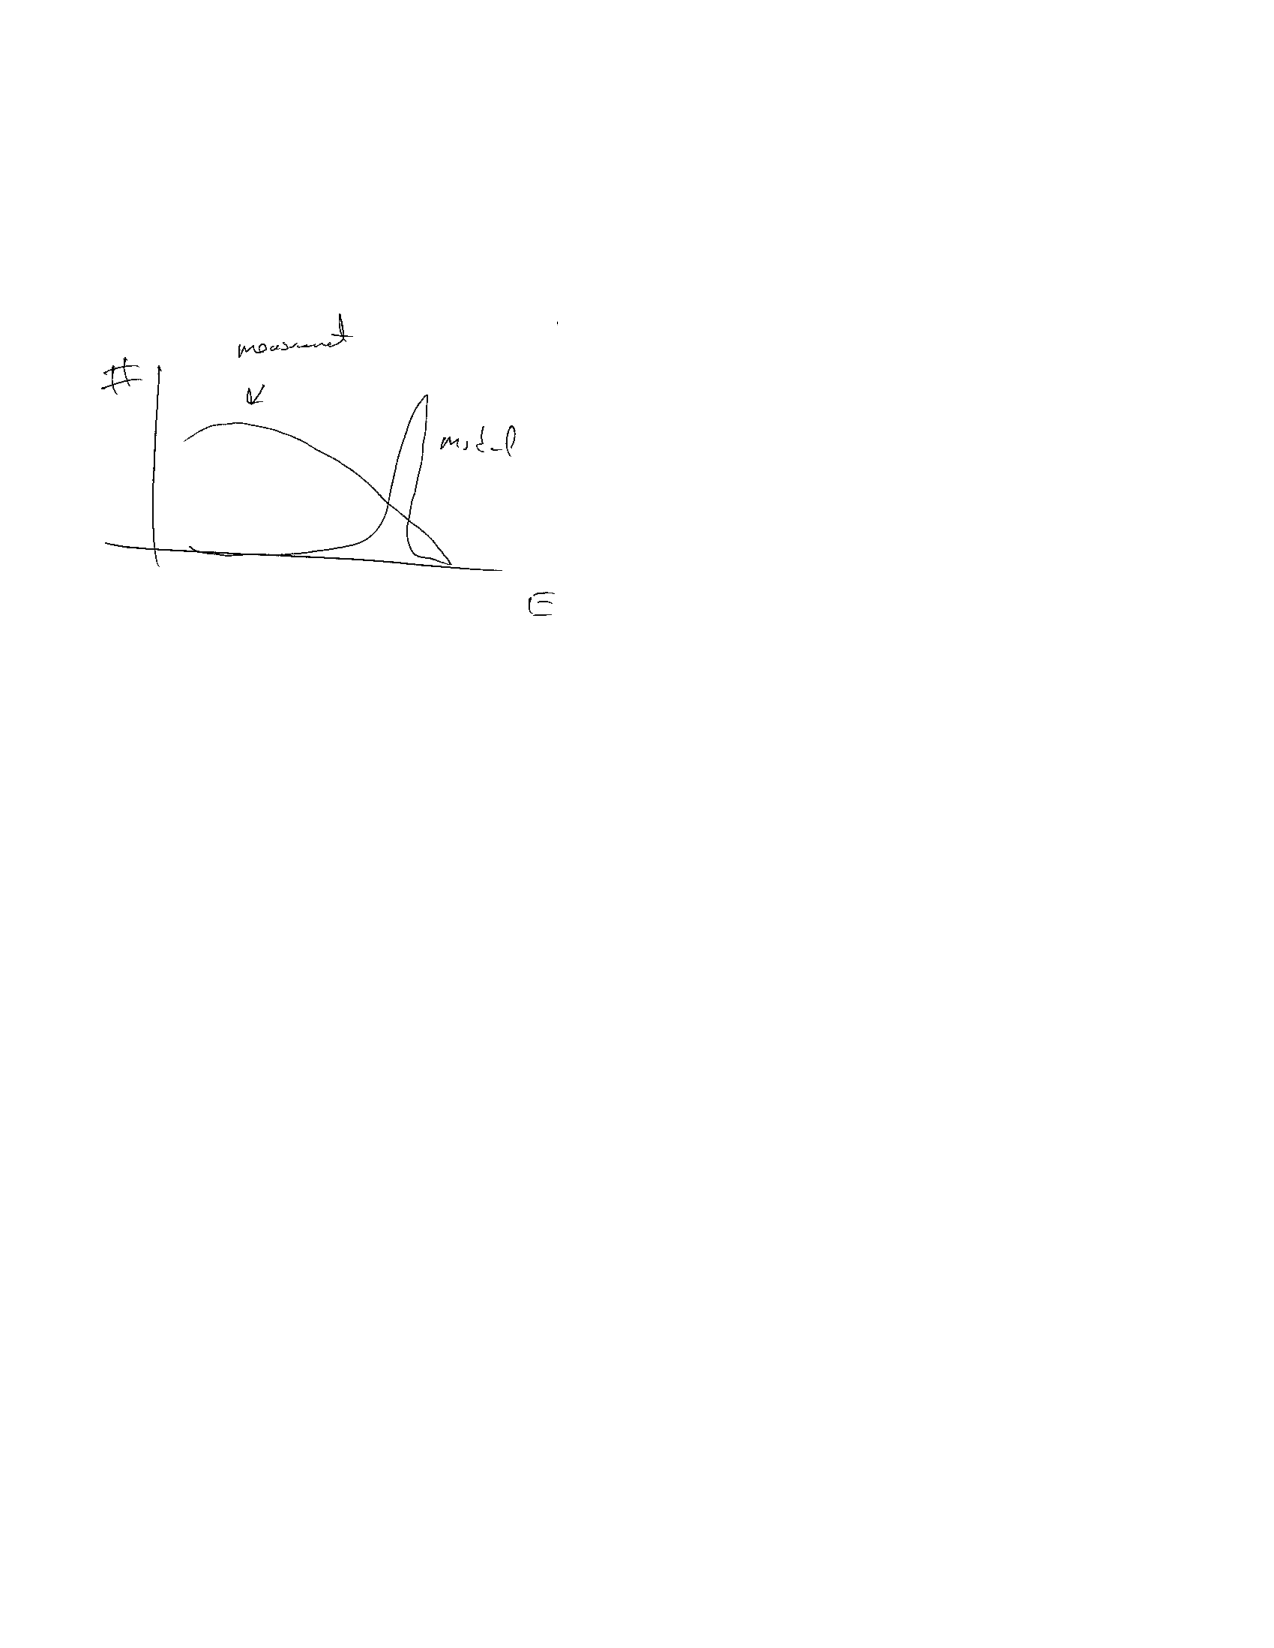
\includegraphics[width=0.7\textwidth]{./CountsVsE.pdf}
\end{figure}

The question is what happened ? 
There is an obvious answer, you have losses somewhere. 
However clever experimentalists convinced everybody that this was not the case. 
(e.g. can test this by using thing targets or measuring if the sample heats up)  

$\Rightarrow$ fundamental $\beta$ spectrum is \underline{Continuous}.

\textbf{\underline{Elsewhere, in the mean time} }

People where hard at work figuring out what was going on with radiation

They had come-up with very good models for $\alpha$ and $\beta$ radiation. 

\begin{center}
$\alpha$ : N $\rightarrow$ N' + N$_{\textrm{He}}$

$\beta$ : N $\rightarrow$ N' + e
\end{center}

These models worked very well and they made predictions. 
In particular they predicted that the $\beta$ decay was a 2-body decay. 
So given the masses of the two nuclei, the electrons energy is well-defined. 
This of course is in disagreement with the measured spectrum, so clearly there is something fundamentally wrong with our model. 

This was the situation in the 1920s...

At the same time, people were trying to figure out what nuclei are. 
We knew that nuclei had substructure. 
A big hint was that they could do complicated stuff like radiation.   

\textbf{\underline{Nuclear physics in the 20's}} (again remember here we are still figuring out QM)

Had a very good model of the nucleus

0th order:  N = $n_p$p + $n_e$e

Nuclei can spit out electrons, so these must be there as well.  
There are some (unknown) interactions that keep things together, and every once in a while some subset of these can leave the nucleus. 

This was a very good model. 

For example, 

\begin{center}
$^{4}$He = 4p + 2e$^-$ which worked very well
\end{center}

however 

\begin{center}
$^{14}$N = 14p + 7e$^-$ made some disturbing predictions.   
\end{center}

We now understand $^{14}$N to be made of 7n + 7p = (14 spin 1/2 fermions), which makes $^{14}$N a boson

The 20s nuclear model predicts $^{14}$N to be fermion (14 + 7 spin 1/2 fermions)

So this model made a prediction which was wrong. 

Big problem... another was with magnetic moments. 

\be
\mu \propto \frac{e}{m}  \hspace{0.2in} \textrm{so,  }\ \mu_e >> \mu_p
\ee
B/c the electron mass is so much smaller. 

This predicts that the nuclear magnetic moments should be dominated by the electrons. 

However what was seen was 
\be
\mu_N \sim \mu_p << \mu_e \hspace{0.2in} \textrm{which again does not fit with $^{14}$N}
\ee

This was exciting times in particle physics! 

Turns out the solution to all these problems was the neutrino.

\textbf{\underline{Early days of \nus}}

\textbf{- 1930:} Pauli invents the neutrino (Takes the 1920s nuclear model and makes it a little more complicated )

Now a nucleus is

\begin{center}
N = $n_p$p + $n_e$e + $n_\nu \nu$
\end{center}

To save the successes of the previous model, the new particle had to be 1) neutral 2) light, 3) spin-1/2 and -- to avoid having seen it already -- 3) weakly interacting. 

(this model doesn't fix the magnetic moment problem ... )

But it explains $\beta$ radiation as well.

Now the model for $\beta$ radiation is

\begin{center}
N $\rightarrow$ N' + e + $\nu$
\end{center}

So the energy of the electron isn't fixed b/c there is another particle that you don't observe taking energy away.

Pauli saw this hypothesis as a ``desperate way out''.
He actually felt bad that he predicted a particle that could not be detected. 

But it was a fantastic idea, which turned out to be correct! 


\textbf{- 1932:} Chadwick  discovers the neutron. This of course is not Pauli neutral particle (too heavy) but changed the way we understood nuclei in a major qualitative way . 

\textbf{- 1934:} We get Fermi's theory of the weak interactions.  We have already talked in this course about how much of a big deal this was. 
It was Bold and did things that no other theory before had done. 

Will pick up here next time....


}
\end{document}


